\documentclass[11pt,a4paper]{article}
\usepackage[T1]{fontenc}
\usepackage[utf8]{inputenc}
\usepackage{lmodern}
\usepackage[margin=26mm]{geometry}
\usepackage{amsmath,amssymb,amsthm,booktabs,microtype,graphicx}
\usepackage[hidelinks]{hyperref}
\usepackage{xurl}
\setlength{\emergencystretch}{1.5em}
\newtheorem{theorem}{Theorem}
\newtheorem{lemma}[theorem]{Lemma}
\newtheorem{corollary}[theorem]{Corollary}
\newtheorem{proposition}[theorem]{Proposition}
\theoremstyle{remark}
\newtheorem{remark}[theorem]{Remark}
\DeclareMathOperator{\diag}{diag}
\newcommand{\one}{\mathbf 1}
\newcommand{\R}{\mathbb R}
\title{When mixing lowers similarity-sensitive entropy\\[3pt]
\large Exact concavity criteria and sharp bounds on entropy gain}
\author{Anonymous}
\date{November 2026\\[2pt]\small DOI \href{https://doi.org/10.5281/zenodo.24514480}{10.5281/zenodo.24514480}}
\begin{document}
\maketitle
\begin{abstract}
Similarity-sensitive entropy measures the uncertainty, or diversity, of a distribution when some outcomes count as partly alike. It is used to partition ecological diversity, to define information gain in Bayesian experimental design and to build divergences in machine learning. Each of these uses needs the entropy to be concave: pooling two populations, or averaging over what an experiment might reveal, should never lower it. Concavity can fail, and earlier work gave counterexamples and posed exact questions. We give a finite test that decides concavity for any finite similarity matrix: after identical rows are merged, the matrix must be positive definite and one explicit matrix per state must be positive semidefinite. For positive definite similarities satisfying the multiplicative triangle inequality, four states never permit failure and five can, which answers Miller's minimum-cardinality question. We also bound how large a failure can be. With $n$ states and a similarity that is positive semidefinite or satisfies the multiplicative triangle inequality, the expected entropy after an observation can exceed the entropy before it by at most $\tfrac12\log n$; for positive semidefinite similarities the sharp worst case is $\tfrac12\log n-\log\log n+\log 2-1+o(1)$. Further results classify the pairs of similarities whose joint entropy is subadditive, give a linear-time test on weighted trees and a safe class containing all ultrametric similarities, and show that among average-rarity indices only Rao's quadratic entropy is concave for every positive definite metric similarity. The paper ends with practical guidance on which similarity matrices are safe.
\end{abstract}

\section{Introduction}\label{sec:intro}
This section explains the problem, why it matters, what was known, and what this paper adds.

\paragraph{The problem.} Suppose there are $n$ possible outcomes, such as species in a community, labels in a classification task or hypotheses in a forecast. A similarity matrix $K$ records how alike each pair of outcomes is, on a scale from zero (unrelated) to one (identical). For a probability distribution $p$ on the outcomes, the \emph{typicality} of outcome $i$ is $(Kp)_i$, the expected similarity between $i$ and a random draw from $p$. The similarity-sensitive entropy of order one is
\[
 H_K(p)=-\sum_i p_i\log (Kp)_i ,
\]
the mean of minus the log typicality. When $K$ is the identity it is Shannon entropy. Leinster and Cobbold \cite{lc} introduced $\exp H_K$ as an effective number of distinct types, and the same functional appears as the order-one index of Ricotta and Szeidl \cite{rs}, as Bavaud's reduced entropy \cite{bavaud}, and as the order-one GAIT entropy of Gallego Posada et al.\ \cite{gait}.

\paragraph{Why concavity matters.} Three uses of $H_K$ rely on concavity, that is on $H_K(\lambda p+(1-\lambda)r)\ge\lambda H_K(p)+(1-\lambda)H_K(r)$.
\begin{itemize}
\item In ecology, the diversity of two pooled communities should be at least their average diversity. Partitions of diversity into within-community (alpha) and between-community (beta) parts assume this \cite{botta,reeve}; a beta-diversity below one is then uninterpretable.
\item In Bayesian inference and experimental design, an observation should not raise the expected uncertainty about the outcome. Miller \cite[Section 4.1]{miller} notes that this holds for every prior and every observation exactly when $H_K$ is concave, and proposes the expected entropy reduction as a design utility \cite[Section 6.2]{miller}.
\item In machine learning, the GAIT divergence \cite[Definition 2]{gait} is the Bregman remainder of $-H_K$. It is nonnegative, and the associated scoring rule is proper, only when $H_K$ is concave.
\end{itemize}

\paragraph{What was known.} Concavity is not automatic. Gallego Posada et al.\ computed the Hessian of $H_K$, proved concavity for two states and conjectured it for every positive definite $K$ satisfying the multiplicative triangle inequality (MTI) $K_{ik}\ge K_{ij}K_{jk}$ \cite[Conjecture 1 and Supplement C]{gait}. Bavaud gave a three-state failure that violates that inequality, showed that subadditivity can also fail, and asked for the exact conditions under which reduced entropy is concave or subadditive \cite[Section 6]{bavaud}. Miller proved concavity for Laplace kernels on the real line, refuted the conjecture with an 18-state example, and asked for the least number of states that permits failure under the two hypotheses \cite[Section 6.2 and Appendix E]{miller}. For the wider Ricotta--Szeidl family of indices, the claim of concavity for orders at least two \cite[Theorem 2]{rs} was later acknowledged to rest on a faulty proof, with numerical evidence that only order two is concave in general \cite{rsp}.

\paragraph{What is new.} The paper makes the following contributions.
\begin{enumerate}
\item A finite test (Theorem~\ref{th:main}). $H_K$ is concave if and only if, after identical rows are merged, the reduced matrix $L$ is positive definite and $m$ explicit \emph{vertex matrices} are positive semidefinite. The proof turns the known Hessian into a matrix that is affine in $p$. When the test passes, concavity is strict on reduced laws. A sufficient sign condition (Corollary~\ref{cor:sign}), extending Miller's line argument, covers every ultrametric similarity.
\item The exact minimum (Theorem~\ref{th:min}). Every similarity on at most four states satisfying the multiplicative triangle inequality has concave entropy, and a five-state positive definite example on the complete bipartite graph $K_{2,3}$ fails. The four-state step uses an exact polynomial certificate.
\item Weighted trees (Proposition~\ref{prop:trees}). The test reduces to one matrix and runs in linear time. Stars fail exactly beyond an explicit number of leaves, a star with equal edges needs at least 13 states to fail, and minimal failing examples can be arbitrarily large.
\item The size of a failure (Theorem~\ref{th:half}). If $K$ is positive semidefinite or satisfies MTI, the excess of expected posterior entropy over prior entropy is at most half the expected posterior entropy, hence at most $\tfrac12\log n$. Over positive semidefinite similarities the worst case is $\tfrac12\log n-\log\log n+\log 2-1+o(1)$, attained by a binary observation. A by-product (Proposition~\ref{prop:effective}) is that Bavaud's effective entropy, which is always concave, lies between one half and all of $H_K$.
\item Subadditivity (Theorem~\ref{thm:subadd}). Joint entropy under the tensor-product similarity is subadditive for every joint law exactly when one factor is the all-ones matrix, or a partition with at least two classes and the other entropy is concave. This answers the second part of Bavaud's question.
\item Other rarity profiles (Theorem~\ref{thm:rarity}). Among indices $\sum_ip_i\phi((Kp)_i)$, only affine nonincreasing $\phi$ are concave for every positive definite metric similarity. In the Ricotta--Szeidl family this leaves only Rao's quadratic entropy, and every other order fails on six states.
\item Infinite spaces (Theorem~\ref{thm:restriction}). On a standard Borel space, $H_K$ is concave if and only if every finite restriction is, with an explicit bias bound for the empirical plug-in estimator.
\end{enumerate}
Several facts used along the way are known and are credited where they appear: the Hessian \cite{gait}, the equivalence between concavity and nonnegative expected information gain \cite{miller}, Bavaud's derivative at product laws and modularity identity \cite{bavaud}, and positive definiteness of four-point metric spaces \cite{meckes}.

\paragraph{Roadmap.} Section~\ref{sec:setting} fixes notation. Section~\ref{sec:criterion} proves the finite test and the sign condition. Section~\ref{sec:consequences} records what the test decides for conditioning, divergences and coarse-graining. Section~\ref{sec:min} settles the minimum number of states, and Section~\ref{sec:trees} treats trees. Section~\ref{sec:mixing} bounds the size of a failure. Sections~\ref{sec:subadd}, \ref{sec:rarity} and~\ref{sec:measure} treat subadditivity, other indices and infinite spaces. Section~\ref{sec:practice} gives practical guidance and Section~\ref{sec:discussion} lists open problems.

\section{Setting and notation}\label{sec:setting}
This section collects the definitions used throughout.

A \emph{similarity matrix} is a symmetric matrix $K\in[0,1]^{n\times n}$ with $K_{ii}=1$. A \emph{law} is a probability vector $p$ in the simplex $\Delta_n=\{p\ge0:\one^\top p=1\}$. The \emph{typicality} vector is $q=Kp$. Since $q_i\ge p_i$, the entropy
\begin{equation}\label{eq:H}
 H_K(p)=-\sum_{i:p_i>0}p_i\log q_i
\end{equation}
is continuous on the closed simplex; logarithms are natural. $K$ is \emph{positive definite} (PD) or \emph{positive semidefinite} (PSD) in the usual matrix sense, and satisfies the \emph{multiplicative triangle inequality} (MTI) if
\begin{equation}\label{eq:mti}
 K_{ik}\ge K_{ij}K_{jk}\qquad (i,j,k\in\{1,\ldots,n\}).
\end{equation}
For positive entries, MTI says exactly that $d_{ij}=-\log K_{ij}$ obeys the triangle inequality, so $K=e^{-d}$ for a metric $d$; we then call $K$ a \emph{metric similarity}.

\emph{Reduction.} Partition the indices into classes of identical rows and keep one representative per class; by symmetry the corresponding columns also agree. Let $L$ be the principal submatrix on the representatives and $m$ its order. If $\pi$ is the vector of class masses of $p$, then $H_K(p)=H_L(\pi)$. We write $e_j$ for a coordinate vector and $D(z)=\diag(z)$.

\emph{Observations.} An observation (or experiment) about the outcome produces a random posterior law $P$ whose mean is the prior $p=\mathbb E P$. It is \emph{binary} when $P$ takes two values and \emph{fair} when these have probability one half each. Any binary mixture $p=\lambda p'+(1-\lambda)p''$ arises from the binary observation that reveals which component was drawn. Concavity of $H_K$ is therefore the statement that $\mathbb E H_K(P)\le H_K(p)$ for every observation.

\section{A finite test for concavity}\label{sec:criterion}
This section proves that concavity is decided by finitely many semidefiniteness checks, one for each state of the reduced matrix.

\begin{theorem}\label{th:main}
The function $H_K$ is concave on $\Delta_n$ if and only if $L$ is positive definite and all $m$ \emph{vertex matrices}
\begin{equation}\label{eq:test}
 T_j=L^{-1}D(Le_j)+D(Le_j)L^{-1}-e_je_j^\top,\qquad 1\le j\le m,
\end{equation}
are positive semidefinite. When these conditions hold, $H_L$ is strictly concave. Equality in a nontrivial mixture of two laws occurs exactly when their class masses agree. In particular, $H_K$ itself is strictly concave precisely when it is concave and its rows are distinct.
\end{theorem}

\begin{proof}
We first work with the original kernel. Extend $F(p)=-H_K(p)$ by the same formula to the open positive cone. For $q=Kp$ and $w=Kv$, direct differentiation gives
\begin{equation}\label{eq:hess}
 B_p(v,v)=v^\top\nabla^2F(p)v
 =2\sum_i v_i w_i/q_i-\sum_i p_i(w_i/q_i)^2.
\end{equation}
This is the Hessian of \cite[Supplement C.2]{gait}. Polarisation gives $B_p(p,v)=\one^\top v$ and $B_p(p,p)=1$. At an interior law write $v=v_0+(\one^\top v)p$ with $\one^\top v_0=0$. Then $B_p(v,v)=B_p(v_0,v_0)+(\one^\top v)^2$, so the Hessian is positive semidefinite on the tangent space of the simplex exactly when it is positive semidefinite on all of $\R^n$. Convexity of $F$ on the open simplex extends to the closed simplex by continuity of~\eqref{eq:H}.

\emph{Necessity of positive definiteness.} Suppose $F$ is convex. If $Kv=\lambda v$ with $\lambda<0$, both terms on the right of \eqref{eq:hess} are negative at every interior law, so $K$ is positive semidefinite. If $v\in\ker K$, then $B_p(v,v)=0$, so positive semidefiniteness of $B_p$ forces $B_p(v,u)=0$ for all $u$. By \eqref{eq:hess} this says $KD(q)^{-1}v=0$: the diagonal matrix $D(q)^{-1}$ preserves $\ker K$, and by symmetry also $\operatorname{range} K$. Choose a positive law $p$ for which $(Kp)_i\ne(Kp)_k$ whenever rows $i,k$ differ. Such laws exist: if $K_{i\cdot}-K_{k\cdot}$ is a nonzero multiple of $\one^\top$ the equality is impossible on the simplex, and otherwise it defines a proper hyperplane. The spectral projections of $D(q)^{-1}$ are then the projections onto the row classes; they are polynomials in $D(q)^{-1}$ and therefore preserve $\operatorname{range}K$. This range contains $q$, which is positive and constant on each class, so it contains every class indicator. Conversely every vector in the range is constant within classes. Hence the range has dimension exactly $m$. Writing $K=ULU^\top$, with $U$ the class-indicator matrix, shows that $L$ has rank $m$ and is positive definite.

\emph{The vertex matrices.} Now use the reduced kernel $L$ and a positive law $p\in\Delta_m$. Put $A=L^{-1}$, $q=Lp$ and $y=D(q)^{-1}Lv$; every $y\in\R^m$ occurs. Substituting $v=AD(q)y$ in \eqref{eq:hess} gives
\begin{equation}\label{eq:affine}
 B_p(v,v)=y^\top\big[A D(Lp)+D(Lp) A-D(p)\big]y
 =y^\top\Big(\sum_j p_j T_j\Big)y.
\end{equation}
The bracket is affine in the law. It is positive semidefinite at every interior law if and only if it is so at the vertices, by convex combinations in one direction and limits in the other. No division at a vertex is needed even when $L$ has zero entries. The factorisation through class masses transfers both directions to $K$.

\emph{Strictness.} Write $k_j=Le_j$, $k_j^{\circ 2}$ for its entrywise square and $L\circ L$ for the entrywise square of $L$. Since $Ak_j=e_j$ and $(k_j)_j=1$,
\[
 T_j k_j=A k_j^{\circ 2},\qquad k_j^\top T_j k_j=1.
\]
The Cauchy--Schwarz inequality for the positive semidefinite form $T_j$ gives $T_j\succeq A k_j^{\circ 2}(k_j^{\circ 2})^\top A$. Consequently
\[
 \sum_j p_jT_j\succeq A(L\circ L)D(p)(L\circ L)A\succ0
\]
at every positive law, because $L\circ L$ is a principal submatrix of the positive definite matrix $L\otimes L$. Thus $F$ has positive definite Hessian on the reduced interior. On a segment joining two distinct laws, restrict to the union of their supports. Concavity passes to that face, the corresponding principal submatrix of $L$ is positive definite, and the same argument gives strictness in the relative interior of the segment. Lifting back through class masses proves the equality assertion.
\end{proof}

For rational input the test uses exact arithmetic throughout. Dense elimination costs $O(m^4)$ arithmetic operations for all $m$ tests after reduction, not counting bit growth. The test decides necessity as well as sufficiency, with no sign restriction on $L^{-1}$. A simple sufficient condition follows from Miller's proof for Laplace kernels on the line \cite[Appendix B.1]{miller}, whose argument uses only the signs of the inverse.

\begin{corollary}\label{cor:sign}
Suppose the reduced matrix $L$ is invertible, $A=L^{-1}$ has nonpositive off-diagonal entries and every row sum of $A$ is nonnegative. Then $H_K$ is concave. This holds for every ultrametric similarity, that is every similarity with $K_{ij}\ge\min(K_{ik},K_{kj})$ for all $i,j,k$. It also holds for every Laplace kernel $e^{-|x_i-x_j|}$ on distinct real points.
\end{corollary}
\begin{proof}
Write $r_i=\sum_jA_{ij}\ge0$ and $w_{ij}=-A_{ij}\ge0$ for $i\ne j$. For a law $p$ with typicalities $q=Lp$ we have $p=Aq$, that is $p_i=r_iq_i+\sum_{j\ne i}w_{ij}(q_i-q_j)$. Substituting and grouping pairs gives Miller's identity \cite[Appendix B.1]{miller}
\[
 -H_L(p)=\sum_ir_iq_i\log q_i+\sum_{i<j}w_{ij}(q_i-q_j)\log\frac{q_i}{q_j}.
\]
Each term is a convex function of $q$: $t\log t$ is convex, and $(a-b)\log(a/b)$ is jointly convex by the log-sum inequality. As $q$ is a linear function of $p$, $H_L$ is concave, and so is $H_K$. An ultrametric similarity satisfies MTI, since $\min(K_{ik},K_{kj})\ge K_{ik}K_{kj}$. So identical rows can be merged (Theorem~\ref{th:main}) and zero similarities split the states into blocks whose entropies combine concavely (Lemma~\ref{lem:blocks} below). On a block with distinct rows, $d=-\log K$ is a proper ultrametric and Bavaud \cite[Theorem 6c]{bavaud} shows that $L^{-1}$ is a strictly diagonally dominant Stieltjes matrix, which has the required signs. For the Laplace kernel the signs are computed in \cite[Appendix B.1]{miller}.
\end{proof}

\section{What the test decides}\label{sec:consequences}
This section records the known properties that are equivalent to concavity, so that Theorem~\ref{th:main} decides each of them for a given matrix.

For a fixed finite kernel, conditioning has nonnegative mean information gain for every prior and observation if and only if $H_K$ is concave: Jensen's inequality gives one direction and a binary observation the other. Miller states both directions for this entropy \cite[Section 4.1 and Lemma A.1]{miller}. For interior laws $p,r$ the GAIT divergence is the remainder $F(p)-F(r)-\nabla F(r)^\top(p-r)$ for $F=-H_K$ \cite[Definition 2]{gait}. By the first-order characterisation of convexity it is nonnegative for every such pair exactly when $H_K$ is concave, and under concavity it vanishes exactly when the reduced class masses agree. Equivalently, the tangent scoring loss is proper on interior reports and strictly proper on reduced states, as Miller notes for concave $H_K$ \cite[Section 6.2]{miller}. The new point is only that each property can now be checked from the matrix by Theorem~\ref{th:main}. Equation~\eqref{eq:gap} below gives an explicit binary observation that raises the expected entropy.

Miller also asks how concavity behaves under a change of representation \cite[Section 6.2]{miller}. For a deterministic map of finite sets with a full-support input law, his induced similarity between distinct outputs is the largest input similarity across their fibres \cite[Definition 3.3]{miller}. The next observation shows that this construction, applied to the safest input kernels, can produce every positive output similarity.

\begin{proposition}\label{prop:induced}
Every finite similarity matrix $K$ with $0<K_{ij}<1$ for $i\ne j$ is induced by a deterministic map from a finite subset of the real line with similarity $\exp(-|x-y|)$ and a full-support input law.
\end{proposition}
\begin{proof}
The one-state case is immediate. For each unordered pair $\{i,j\}$ choose a separate cluster of two real points at distance $-\log K_{ij}$, labelled $i$ and $j$. Separate consecutive clusters by gaps greater than $\max_{i\ne j}(-\log K_{ij})$, and map each point to its label. The smallest distance between the fibres of $i$ and $j$ is attained inside their own cluster and equals $-\log K_{ij}$, so the largest cross-fibre similarity is $K_{ij}$. The uniform law has full support.
\end{proof}

Miller's line theorem \cite[Theorem 4.4]{miller} gives concavity on the input. The proposition shows that this alone puts no restriction on the output matrix; in particular the five-state example of Section~\ref{sec:min} is attainable. Theorem~\ref{th:main}, applied to the induced matrix, decides whether conditioning can raise entropy on the output space.

\section{Four states are safe, five are not}\label{sec:min}
This section answers Miller's question: what is the least number of states on which a positive definite similarity satisfying MTI can have nonconcave entropy?

\begin{theorem}\label{th:min}
\begin{enumerate}
\item[(a)] Every similarity matrix of order at most four satisfying MTI has concave entropy, with equality in a nontrivial mixture exactly when the two laws assign equal mass to each class of identical rows. No positive definiteness assumption is needed.
\item[(b)] There is a positive definite similarity matrix of order five satisfying MTI whose entropy is not concave.
\end{enumerate}
Hence five is the minimum order for which positive definiteness and MTI fail to guarantee concavity.
\end{theorem}

\subsection{Five states suffice for failure}\label{sec:five}
Divide five states into two parts, of two and three states. Put one on the diagonal, $a^2$ between distinct states of the same part, and $a$ across the parts, where $0<a<1$. This is $K_{ij}=a^{d_{ij}}$ for the shortest-path distance on the complete bipartite graph $K_{2,3}$, so it satisfies \eqref{eq:mti}. Vectors summing to zero inside one part and vanishing on the other have eigenvalue $1-a^2$. On the two normalised part indicators the matrix is
\[
 \begin{pmatrix}1+a^2&\sqrt6\,a\\ \sqrt6\,a&1+2a^2\end{pmatrix},
 \qquad\det=(1-a^2)(1-2a^2).
\]
So $K$ is positive definite exactly when $a<1/\sqrt2$. This graph is the classical five-point metric space that is not of negative type; its similarity matrix becomes singular at $a=1/\sqrt2$ \cite[Example 2.2.7]{leinster-mag}, \cite[Section 3.2]{meckes}.

Let $P$ and $Q$ be the uniform laws on the two parts and $M=(P+Q)/2$. Within their own parts the mean similarities are $\alpha=(1+a^2)/2$ and $\beta=(1+2a^2)/3$; across the parts the mean is $a$. The fair binary observation that reveals the part therefore raises expected entropy by
\begin{equation}\label{eq:gap}
 J=\frac{H_K(P)+H_K(Q)}2-H_K(M)
  =\frac12\log\frac{(\alpha+a)(\beta+a)}{4\alpha\beta}.
\end{equation}
Choose $a=12/17$. Then $1-2a^2=1/289>0$ and
\[
   J=\tfrac12\log(999949/999364)\approx0.00029260\text{ nats}>0 .
\]
This proves failure on the closed simplex, and by continuity the strict gap persists after adding a small amount of uniform mass to both posteriors. Figure~\ref{fig:five} shows the whole mixture segment. As a direct interior check at $a=7/10$, take $p=(36,1,1,1,1)/40$ and $v=(2,1,-1,-1,-1)$. The second derivative of $H_K$ along $p+tv$ at $t=0$ is $+2748940385160/93148730546881>0$; equation \eqref{eq:hess} gives the negative of this number for $F=-H_K$.

\begin{figure}[ht]\centering
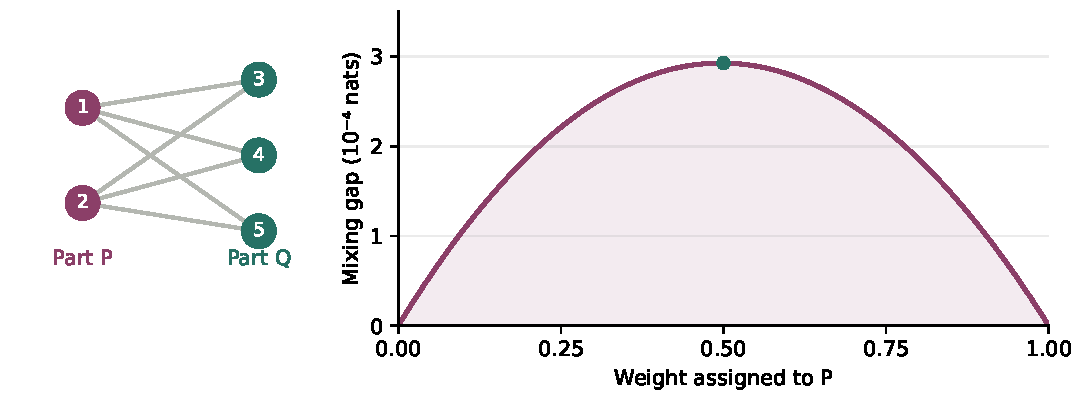
\includegraphics[width=0.89\linewidth]{figures/mixing-example.pdf}
\caption{The five-state kernel at $a=12/17$ and its mixing gap. The left panel shows the graph $K_{2,3}$; similarity is $a$ across an edge and $a^2$ between states of the same part. The right panel plots the weighted mean of the two part entropies minus the entropy of the mixture, as the weight on part $P$ varies. Concavity would require this curve to lie at or below zero; positive values are failures.}
\label{fig:five}
\end{figure}

The failure persists over an interval of edge similarities; the proof uses the vertex Schur complement \eqref{eq:schur} defined in Section~\ref{sec:four}. At a root in the two-state part, that Schur complement splits into the two contrasts within the three-state part and a two-dimensional block. The block has diagonal entries $2/a^2-1-a^4$ and $2/a-2a-3(1-a)^2$ and off-diagonal entry $\sqrt3(1-a^4)/a$. Its determinant is
\[
 -\frac{(1-a)^2(1+a)}{a^3}
 (4a^5+a^4+7a^3-5a^2+5a-4).
\]
The polynomial in parentheses is strictly increasing on $(0,1)$, since its derivative $20a^4+4a^3+21a^2-10a+5$ is positive, and it changes sign between $0.673$ and $0.674$. Thus throughout the open interval from its root ($\approx0.673648$) to $1/\sqrt2$, $K$ remains positive definite while its entropy fails concavity. The exact classifier agrees with this interval on the grid $a=0.60,0.61,\ldots,0.70$. The interval has width about $0.033$ and lies just below the value at which $K$ stops being positive definite.

\subsection{Four states never fail}\label{sec:four}
We first record that four-point metric similarities are positive definite, then prove concavity in four cases.

\begin{lemma}\label{lem:pd4}
If $d$ is a metric on at most four distinct points, then $K=e^{-d}$ is positive definite.
\end{lemma}
\begin{proof}
This is part of \cite[Theorem 3.6(4)]{meckes}: such spaces are of negative type and hence positive definite. A self-contained proof uses the cut decomposition below. With weights $u_\ell\ge0$ on cuts $\ell$, $K_{xy}=\prod_\ell e^{-u_\ell|\sigma_\ell(x)-\sigma_\ell(y)|}$, where $\sigma_\ell(x)\in\{0,1\}$ records the side of cut $\ell$ containing $x$. So $K$ is a principal submatrix of the tensor product of the $2\times2$ matrices with diagonal one and off-diagonal $e^{-u_\ell}$ over the cuts with $u_\ell>0$. Each factor is positive definite, and distinct points have distinct bit vectors because their distance is positive. Metrics on fewer than four points extend to four points by attaching a leaf at positive distance, and $K$ is then a principal submatrix.
\end{proof}

\emph{Case 1: four distinct states, all similarities positive.} At the vertex with root $0$, let $k_i=K_{i0}$. By \eqref{eq:hess} the full Hessian of $F$ there is $M_{ij}=K_{ij}(1/k_i+1/k_j)-k_i k_j$. Its root row and column consist of ones. Taking the Schur complement of $M_{00}=1$ yields
\begin{equation}\label{eq:schur}
 C_{ij}=K_{ij}(1/k_i+1/k_j)-k_i k_j-1,\qquad i,j\in\{1,2,3\}.
\end{equation}
By Lemma~\ref{lem:pd4} $K$ is positive definite, and $k_i>0$, so the change of variables in \eqref{eq:affine} is invertible at this vertex. Hence $C\succeq0$ is equivalent to the vertex test $T_0\succeq0$.

The distances $d_{ij}=-\log K_{ij}$ form a metric. On four points every metric is a nonnegative combination of cut distances \cite{dl}; we give the coefficients so that the certificate is explicit. A cut distance is one between different sides of a partition and zero within either side. Permute the three nonroot labels so that $S_1=d_{01}+d_{23}$ is the largest of $S_1$, $S_2=d_{02}+d_{13}$ and $S_3=d_{03}+d_{12}$; this is possible because the root is fixed and each of the three pairings contains it. The cut $01|23$ then has weight zero. The cuts $02|13$ and $03|12$ have weights $(S_1-S_2)/2$ and $(S_1-S_3)/2$. The singleton cuts at $0,1,2,3$ have weights equal to half of
\[
 d_{02}+d_{03}-d_{23},\quad d_{12}+d_{13}-d_{23},\quad
 d_{02}+d_{12}-d_{01},\quad d_{03}+d_{13}-d_{01}.
\]
All weights are nonnegative, and summing the weights of the cuts that separate each pair recovers the six distances (checked symbolically in \texttt{check\_extensions.py}).

We now show that all seven principal minors of \eqref{eq:schur} are nonnegative. Represent each of the six cuts by its bit vector with first bit zero, omitting $0000$ and $0011$, in lexicographic order. For a cut weight $u_\ell$ put $b_\ell=e^{u_\ell}=1+t_\ell$ with $t_\ell\ge0$. Let $s_{ij}\in\{0,1\}^6$ indicate the cuts separating $i$ and $j$, and put $s_i=s_{0i}$. Then $K_{ij}=b^{-s_{ij}}$ in multi-index notation, and \eqref{eq:schur} becomes
\[
 C_{ij}=b^{s_i-s_{ij}}+b^{s_j-s_{ij}}-b^{-s_i-s_j}-1 .
\]
Expand each principal minor $P_I=\det C_{I,I}$ by permutations. For each variable, subtract the smallest exponent present from every exponent of that variable; this removes a positive common Laurent monomial. Expand the result at $b=1+t$ by the binomial theorem. Table~\ref{tab:cert} gives the number and range of its nonzero integer coefficients. Every coefficient is positive, so every $P_I\ge0$ for $t\ge0$, which covers zero cut weights. By the principal-minor criterion $C\succeq0$ for the chosen root. The root was arbitrary, so all four vertex tests pass and Theorem~\ref{th:main} gives strict concavity.

\begin{table}[ht]
\centering\small
\begin{tabular}{lrrr}\toprule
Principal index set $I$ & Nonzero coefficients & Minimum & Maximum\\\midrule
$\{1\}$ &255&2&161\\
$\{2\}$ or $\{3\}$ &63&2&53\\
$\{1,2\}$ or $\{1,3\}$ &1,557&4&3,672\\
$\{2,3\}$ &1,245&4&1,836\\
$\{1,2,3\}$ &15,172&8&464,400\\\bottomrule
\end{tabular}
\caption{Exact certificate for four states, produced by \texttt{verify.py}. The counts depend on the positive monomial normalisation: the independent check \texttt{verify\_independent.py} works with the diagonally congruent matrix $C_{ij}/(k_ik_j)$ and finds different counts (for example 30,562 for $\{1,2,3\}$), again all positive.}\label{tab:cert}
\end{table}

\emph{Case 2: fewer than four distinct states, all similarities positive.} A positive definite positive-entry MTI matrix can be extended one state at a time: for an existing state $j$ add a leaf with column $cKe_j$ and diagonal one, $0<c<1$. This adds an edge of length $-\log c$ at $j$, keeps MTI, and has Schur complement $1-c^2>0$. Restricting the concave four-state entropy to the original face proves concavity, and Lemma~\ref{lem:pd4} with Theorem~\ref{th:main} gives strictness.

\emph{Case 3: identical rows.} MTI makes $K_{ij}=1$ imply that rows $i$ and $j$ coincide, by the two triangle inequalities through these states. Theorem~\ref{th:main} works with the reduced matrix, which again satisfies MTI and has distinct rows.

\emph{Case 4: zero similarities.} The next lemma reduces to blocks of positive similarity.

\begin{lemma}\label{lem:blocks}
If $K$ satisfies MTI then positive similarity is an equivalence relation. On its blocks $b$, with block mass $s_b$ and conditional law $p^{(b)}$,
\[
 H_K(p)=-\sum_b s_b\log s_b+\sum_{b:s_b>0}s_b H_{K_b}(p^{(b)}).
\]
Hence $H_K$ is concave whenever every block entropy $H_{K_b}$ is concave.
\end{lemma}
\begin{proof}
Transitivity of positive similarity is \eqref{eq:mti}. The identity is the modularity property of Leinster and Cobbold, in the form of \cite[Theorem 8]{bavaud}. The first term is Shannon entropy of the block masses, and each other term is the perspective of a concave function, hence concave in $p$.
\end{proof}
Each block has at most four states and positive entries, so Cases 1--3 apply. Equality in a mixture forces equal block masses and, within each block, equal class masses. This proves Theorem~\ref{th:min}(a), and Section~\ref{sec:five} proves part (b).

\begin{remark}
The same threshold appears for Rao's quadratic entropy. Ricotta and Szeidl showed that it is concave for every metric dissimilarity on two, three or four species and left five or more open \cite[Theorem 1 and Remark 1]{rs}. Concavity of Rao's index for a metric is negative type of the metric, so the classical facts that four-point metrics have negative type and $K_{2,3}$ does not \cite[Theorem 3.6 and Section 3.2]{meckes} settle that question too. For the logarithmic entropy no embedding argument is known, and the four-state step relies on the certificate.
\end{remark}

\section{Weighted trees}\label{sec:trees}
This section shows that on tree metrics the $m$ vertex tests collapse into a single matrix condition that can be checked in linear time.

Give each edge $e$ of a finite tree a similarity $0<a_e<1$, and let $K_{ij}$ be the product of the edge similarities along the path from $i$ to $j$. This is the kernel $e^{-d}$ for the tree metric with edge lengths $-\log a_e$. All vertices are states.

\begin{proposition}\label{prop:trees}
Define the symmetric matrix $T$ by
\[
 T_{ii}=2+2\sum_{e\ni i}\frac{a_e^2}{1-a_e^2},\qquad
 T_{ih}=-\frac{\sqrt{a_e}}{1-a_e}\quad(e=ih),
 \qquad T_{ih}=0\quad(i\ne h,\ ih\text{ not an edge}).
\]
Then $H_K$ is concave exactly when $T$ is positive definite and $(T^{-1})_{ii}\le1$ at every vertex. The test takes a linear number of arithmetic operations.
\end{proposition}

\begin{proof}
Root the tree arbitrarily. The precision matrix $A=K^{-1}$ has quadratic form
\[
 x_{\rm root}^2+\sum_{e=(i,h)}\frac{(x_h-a_e x_i)^2}{1-a_e^2},
\]
where $i$ is the parent of $h$. To see this, take independent centred unit-variance innovations at the vertices; set the root equal to its innovation, and each child equal to $a_e$ times its parent plus $\sqrt{1-a_e^2}$ times its innovation. These variables have covariance $K$, and the inverse triangular change of variables gives the displayed form. Thus $A_{ii}=T_{ii}/2$ and $A_{ih}=-a_e/(1-a_e^2)$ on edges.
For the vertex test at $j$, put $k_i=K_{ij}$ and rescale $T_j$ on both sides by $\diag(k_i^{-1/2})$. Across an edge, $k_i/k_h$ is $a_e$ or $a_e^{-1}$, so the rescaled matrix is $T-e_j e_j^{\top}$ at every $j$. If all these matrices are positive semidefinite then $T$ is positive definite, because a null vector of $T$ would have every coordinate zero. For positive definite $T$, the rank-one subtraction satisfies $T-e_j e_j^{\top}\succeq0$ exactly when $(T^{-1})_{jj}\le1$.

For the operation count, root once and eliminate leaves towards the root. A nonpositive pivot rules out positive definiteness. Otherwise compute, for every directed edge $i\to h$, the pivot
\[
 u_{i\to h}=T_{ii}-\sum_{v\sim i,\,v\ne h}T_{iv}^2/u_{v\to i}.
\]
The inward sweep computes the child-to-parent values and the root pivot. An outward sweep computes the reverse messages by caching the full sum at each vertex and omitting its recipient's term. The reciprocal of $T_{ii}-\sum_{v\sim i}T_{iv}^2/u_{v\to i}$ equals $(T^{-1})_{ii}$, by eliminating the components of the tree minus $i$.
\end{proof}

\begin{corollary}\label{cor:star}
On a star with $m$ leaves and common edge similarity $a\in(0,1)$, the entropy is concave exactly when
\[
                 m\le C(a):=\frac{2(1+a)}{a(1-a)}.
\]
Consequently there are positive definite metric similarities of arbitrarily large order whose entropy fails concavity although every proper principal restriction has concave entropy.
\end{corollary}
\begin{proof}
In $T$ the centre has diagonal $c=2+2ma^2/(1-a^2)$, the leaves have diagonal $b=2/(1-a^2)$, and the squared centre--leaf entry is $w=a/(1-a)^2$. The centre Schur complement is $s=c-mw/b=2-m/C(a)$. Positive definiteness requires $s>0$, and the central inverse diagonal is $1/s$, which is at most one precisely when $m\le C(a)$. For such $m$ the inverse diagonal at a leaf is $1/b+w/(b^2s)\le (1-a^2)/2+a(1+a)^2/4=(2+a+a^3)/4\le1$. The centre test therefore decides.
The minimum of $C(a)$ is $6+4\sqrt2\approx11.66$, at $a=\sqrt2-1$, so with a common edge similarity the least failing star has 12 leaves and 13 states. Miller's hub example \cite[Appendix E]{miller} uses a leaf--leaf similarity slightly larger than $a^2$ and exhibits a violation along one family of laws; here the condition is necessary and sufficient over the whole simplex for exact tree similarities.
For any $a$, take $m=\lfloor C(a)\rfloor+1$. Removing a leaf restores the inequality. Removing the centre leaves constant off-diagonal similarity $a^2$, for which the entropy is a sum of the concave scalar functions $-x\log(a^2+(1-a^2)x)$. Further restrictions inherit concavity. Since $C(a)\to\infty$ as $a\downarrow0$, no bound on the size of principal restrictions can certify concavity in all dimensions.
\end{proof}

\section{How much can an observation raise entropy?}\label{sec:mixing}
This section measures the size of a failure. Let $P$ be a random posterior law on $n$ states with mean $p=\mathbb{E}P$, and write
\[
 G=\mathbb{E}H_K(P)-H_K(p)
\]
for the excess of expected posterior entropy over prior entropy, in nats. Concavity is the statement $G\le0$ for every observation.

\begin{theorem}\label{th:half}
Suppose $K$ is positive semidefinite or satisfies MTI. Then
\[
 H_K(p)\ge\tfrac12\mathbb{E}H_K(P),\qquad\text{hence}\qquad G\le\tfrac12\mathbb E H_K(P)\le\tfrac12\log n .
\]
\begin{enumerate}
\item[(a)] Over positive semidefinite similarities and all observations,
\[
 \sup G=\tfrac12\log n-\log\log n+\log 2-1+o(1)\qquad(n\to\infty),
\]
and binary observations attain this.
\item[(b)] Over strictly positive, positive definite tree similarities and fair binary observations, $\sup G\ge\tfrac12\log n-\log\log n-\tfrac52\log2-\tfrac12+o(1)$, while (a) gives $\sup G\le\tfrac12\log n-\log\log n+\log2-1+o(1)$. The ratio $H_K(p)/\mathbb E H_K(P)$ tends to $\tfrac12$ along this family, so the factor $\tfrac12$ is asymptotically optimal even in this class.
\item[(c)] Over MTI similarities without positive semidefiniteness, fair binary observations give $\sup G=\tfrac12\log n+O(1)$.
\end{enumerate}
\end{theorem}

\begin{proof}
\emph{A square-moment bound.} Write $t_q=Kq$ for a law $q$. We first show that for any comparison law $v$,
\begin{equation}\label{eq:square}
 \sum_{i:q_i>0}\frac{q_i t_v(i)^2}{t_q(i)}\le1.
\end{equation}
Under MTI, $t_q(i)\ge K_{ij}t_q(j)$ for each $j$. Hence $\sum_i q_i K_{ij}^2/t_q(i)\le\sum_i q_i K_{ij}/t_q(j)=1$ when $t_q(j)>0$, with sums over the support of $q$; if $t_q(j)=0$ that column vanishes on the support. By convexity of the square, $t_v(i)^2\le\sum_jv_jK_{ij}^2$, and averaging over $j\sim v$ gives \eqref{eq:square}.

Under positive semidefiniteness, write $K_{ij}=\langle g_i,g_j\rangle$ with unit vectors $g_i$ and put $g(v)=\sum_j v_jg_j$. The operator $B_q=\sum_{i:q_i>0} q_i g_i g_i^\top/t_q(i)$ satisfies $B_q\preceq I$. Indeed its nonzero eigenvalues are those of $D^{1/2}K_{SS}D^{1/2}$, where $S=\operatorname{supp}q$ and $D_{ii}=q_i/t_q(i)$ on $S$. This entrywise nonnegative matrix fixes the positive vector with entries $\sqrt{q_it_q(i)}$; conjugating by the diagonal matrix of that vector makes it row-stochastic, so its eigenvalues lie in $[-1,1]$. Therefore
\begin{equation}\label{eq:gram-mean}
 \sum_{i:q_i>0}\frac{q_i t_v(i)^2}{t_q(i)}
 =g(v)^\top B_q g(v)\le\|g(v)\|^2\le1 .
\end{equation}

\emph{The factor one half.} Jensen's inequality for the logarithm in \eqref{eq:square} gives the cross-entropy bound
\begin{equation}\label{eq:cross}
 -\sum_i q_i\log t_v(i)\ge\tfrac12 H_K(q),
\end{equation}
with $+\infty$ allowed on the left. Taking $v=p$ and $q=P$ and averaging proves $H_K(p)\ge\frac12\mathbb EH_K(P)$, since the left side of \eqref{eq:cross} is linear in $q$. As $t_q(i)\ge q_i$, $H_K(q)$ is at most the Shannon entropy of $q$, hence at most $\log n$.

\emph{Upper bound in (a).} Assume $K\succeq0$ and $n\ge2$, and put $L=\log n$. Applying Jensen to \eqref{eq:gram-mean} instead gives $G\le \tfrac12\mathbb E H_K(P)+\log\|g(p)\|$. For large $n$, put $c=L^{-4}$ and $D_L=L-4\log L-1>0$. For a law $q$, let $\delta_q=L-H_K(q)$ and let $U=\{i:t_q(i)>c\}$ have $q$-mass $\theta$. The entropy contribution of $U$ is at most $4\theta\log L$. On its complement $t_q(i)\ge q_i$ and conditional Shannon entropy is at most $L$, so the contribution there is at most $(1-\theta)(L-\log(1-\theta))\le(1-\theta)L+\theta$. Hence $\theta\le\delta_q/D_L$. In the energy $\|g(q)\|^2=\sum_{i,j}q_iq_jK_{ij}$, pairs inside $U$ contribute at most $\theta^2$, and pairs with an endpoint outside $U$ contribute at most $2\sum_{i\notin U}q_it_q(i)\le2c$. Thus $\|g(q)\|\le\theta+\sqrt{2c}$ and
\[
 \|g(p)\|\le\mathbb E\|g(P)\|
 \le\frac{\delta+\eta_L}{D_L},
 \qquad \delta=L-\mathbb{E}H_K(P),\quad
 \eta_L=\sqrt2 D_L/L^2\to0.
\]
Substitution yields
\[
 G\le\tfrac12 L-\log D_L+\log(\delta+\eta_L)-\tfrac12\delta.
\]
For $\eta_L<2$ the last two terms have maximum $\log 2-1+\eta_L/2$ over $\delta\ge0$, at $\delta=2-\eta_L$. Since $\log D_L=\log L+o(1)$, this proves the upper half of (a).

\emph{Lower bound in (a).} Take $m=n-1$ orthonormal leaf vectors and one unit hub vector with inner product $a=(1-1/m)/\sqrt m$ with each leaf. The hub has coordinates $a$ on the leaf directions and $\sqrt{1-ma^2}>0$ on one further direction, so the Gram similarity is positive definite. A binary observation reveals the hub exactly with probability $\lambda=2/\log m$, and otherwise leaves the uniform posterior on the leaves. For $m$ large enough that $\lambda<1$, direct substitution gives
\[
 G=(1-\lambda)\log(1-\lambda+\lambda m a)
      +\lambda\log(\lambda+(1-\lambda)a).
\]
The first logarithm equals $\tfrac12\log m-\log\log m+\log2+o(1)$, and the second term tends to zero. Multiplying the first logarithm by $1-\lambda$ subtracts $1+o(1)$. So the upper bound is attained within $o(1)$. These leaves are mutually orthogonal, so this matrix violates MTI.

\emph{Part (b).} Take two stars with $m$ leaves each and join their hubs by an edge. Give each pendant edge similarity $a=m^{-1/2}$ and the hub edge similarity $b=m^{-2}$. Similarities multiply along paths, so all entries are positive and MTI holds; positive definiteness follows by adjoining leaves one at a time as in Section~\ref{sec:four}. Set $\varepsilon=1/\log m$ and $l=1-\varepsilon$, for $m\ge3$. One posterior puts mass $\varepsilon$ on the first hub and $l/m$ on each leaf of the second star; the other, equally likely, swaps the two stars. Let $c_m=(1+(m-1)a^2)/m$. Under the first posterior an occupied hub and an occupied leaf have typicalities
\[
 u=\varepsilon+l ab,\qquad v=l c_m+\varepsilon ab.
\]
Under the prior every hub has typicality $u_*=(1+b)(\varepsilon+l a)/2$ and every leaf has typicality $v_*=[l(c_m+a^2 b)+\varepsilon a(1+b)]/2$. Thus
\[
 G=\varepsilon\log(u_*/u)+l\log(v_*/v).
\]
Here $u_*/u\to1/2$, $v=2/m+O(\varepsilon/m)$ and $v_*=\varepsilon/(2\sqrt m)\,(1+o(1))$. Hence $l\log(v_*/v)=(1-\varepsilon)(\tfrac12\log m-\log\log m-\log4)+o(1)$, and since $\varepsilon\cdot\tfrac12\log m=\tfrac12$,
\[
 G=\tfrac12\log m-\log\log m-\log4-\tfrac12+o(1),\qquad
 \mathbb E H_K(P)=\log m+O(1).
\]
With $n=2m+2$ states this is the bound in (b), and the ratio of prior entropy to mean posterior entropy tends to $\tfrac12$. For odd $n$ attach one extra leaf with zero probability under both posteriors; this changes neither entropy.

\emph{Part (c).} Use the graph metric of $K_{m,m}$, with $K_{ij}=a^{d(i,j)}$ and $a=m^{-1/2}$, and let a fair binary observation reveal the part of a uniformly drawn state. Each posterior has constant typicality $c_m=(2m-1)/m^2$ on its support, while the prior typicality is $(a+c_m)/2$. Hence
\[
 G=\log\frac{a+c_m}{2c_m}=\tfrac12\log m-\log 4+o(1).
\]
For large $m$ this similarity is indefinite: the contrast between the part indicators has eigenvalue $1+(m-1)a^2-ma<0$. An unused pendant state treats odd $n$. The upper bound $\tfrac12\log n$ completes (c).
\end{proof}

\begin{remark}[Effective range]
The statements of Theorem~\ref{th:half} are asymptotic, and their effective ranges differ. The hub construction is close to the expansion already at moderate size: its excess is within $0.074$, $0.0059$ and $1.3\times10^{-5}$ nats of $\tfrac12\log m-\log\log m+\log2-1$ at $m=10^3$, $10^6$ and $10^{12}$. The upper bound converges slowly; it exceeds the expansion by about $1.8$, $0.45$ and $0.11$ nats at $n=10^6$, $10^{20}$ and $10^{100}$. In the double-star family of (b) the ratio $H_K(p)/\mathbb EH_K(P)$ is $0.92$, $0.66$ and $0.53$ at $m=10^3$, $10^{12}$ and $10^{96}$, so the factor $\tfrac12$ is approached only at very large sizes. These values come from \texttt{check\_extensions.py}.
\end{remark}

The cross-entropy bound \eqref{eq:cross} also compares two diversity indices. Bavaud's effective entropy \cite[equations (6), (13) and (14)]{bavaud} can be written $E(q)=-\sum_{i:q_i>0}q_i\log t_\rho(i)$, where $\rho$ is an optimising law and states of zero mass contribute nothing, and he shows $0\le E\le H_K$. Unlike $H_K$, $E$ is concave for every similarity matrix \cite[Theorem 9]{bavaud}.

\begin{proposition}\label{prop:effective}
If $K$ is positive semidefinite or satisfies MTI, then $\tfrac12H_K(q)\le E(q)\le H_K(q)$ for every law $q$.
\end{proposition}
\begin{proof}
The upper bound is Bavaud's. The lower bound is \eqref{eq:cross} with $v=\rho$.
\end{proof}

So under either hypothesis the always-concave effective entropy is within a factor two of $H_K$. We do not know whether the factor two is attained.

\section{Which product similarities obey subadditivity?}\label{sec:subadd}
This section answers the second half of Bavaud's question: for which pairs of similarities is joint entropy at most the sum of the marginal entropies?

For two finite similarity matrices $K$ and $L$, give the product alphabet the similarity $K\otimes L$. For independent variables the typicalities multiply and the entropies add \cite[Theorem 3]{gait}. Bavaud \cite[Theorem 11 and its proof]{bavaud} derived the first derivative at a product law and remarked that a perturbation can always be chosen to break subadditivity. The next theorem shows that this is true except for one family of pairs, and identifies that family.

\begin{theorem}\label{thm:subadd}
The inequality
\[
 H_{K\otimes L}(P)\le H_K(p)+H_L(r)
\]
holds for every joint law $P$ with marginals $p$ and $r$ precisely for the following pairs, up to interchanging the factors. Either $K$ is the all-ones matrix, or $K$ is the indicator matrix of a partition with at least two classes and $H_L$ is concave. Theorem~\ref{th:main} decides the latter condition even for singular $L$. In the all-ones case equality holds at every law. In the second case equality holds exactly when the class of the first variable is independent of the duplicate-row class of the second.
\end{theorem}

\begin{proof}
Suppose $K_{ij}$ indicates whether $i$ and $j$ belong to the same class. For every class $b$ of positive mass $s_b$, write $r_b$ for the conditional law of the second coordinate. At $(i,k)$ with $i\in b$ the joint typicality equals $s_b(Lr_b)_k$. Thus
\[
 H_{K\otimes L}(P)=H(s)+\sum_{b:s_b>0}s_b H_L(r_b),\qquad H_K(p)=H(s),
\]
where $H(s)$ is the Shannon entropy of the class masses. This is the identity-factor formula of \cite[Theorem 4]{gait} applied to the class label. With a single class there is equality. With at least two classes every binary mixture of second-coordinate laws is realisable, so the inequality is equivalent to concavity of $H_L$, and the equality condition follows from strict concavity on reduced class masses.

Now suppose neither kernel is a partition indicator. We choose principal restrictions and positive laws on them for which both vectors
\[
 \alpha=K\bigl(p/(Kp)\bigr),\qquad \beta=L\bigl(r/(Lr)\bigr)
\]
are nonconstant, with quotients taken coordinatewise. If $K$ has an entry $a\in(0,1)$, use the associated two-state submatrix: as $p$ tends to the first point mass, $\alpha$ tends to $(1,a)^\top$. If $K$ takes only the values zero and one, failure to be a partition supplies a three-state path with two similarities one and end-to-end similarity zero; at the uniform law $\alpha=(5/6,4/3,5/6)^\top$ in path order. Treat $L$ in the same way.

On the restricted alphabets differentiate at the product law $p\otimes r$. The derivative in cell $(i,k)$ is $-\log(Kp)_i-\log(Lr)_k-\alpha_i\beta_k$ \cite[proof of Theorem 11]{bavaud}. A signed $2\times2$ switch preserves both marginals and cancels both logarithmic terms. Choosing two unequal entries of each vector, the directional derivative is $-(\alpha_i-\alpha_j)(\beta_k-\beta_l)\ne0$. One sign of a small switch therefore raises the joint entropy above its value at the product law, which equals the sum of the fixed marginal entropies. Embedding this coupling into the full alphabets by zeros proves failure.
\end{proof}

\section{Which average-rarity indices are concave?}\label{sec:rarity}
This section asks whether replacing the logarithm by another function can restore concavity for all positive definite metric similarities, and shows that only the quadratic choice does.

The order-one entropy belongs to the family
\[
 J_{\phi,K}(p)=\sum_i p_i\,\phi((Kp)_i),
\]
where $\phi$ assigns a rarity to each typicality. Ricotta and Szeidl \cite[Appendix A]{rs} considered the power profiles $\phi_\alpha(x)=(1-x^{\alpha-1})/(\alpha-1)$, with $\phi_1(x)=-\log x$; order two gives Rao's quadratic entropy. They stated that concavity is not expected for $0<\alpha<2$ and asserted it for $\alpha\ge2$ for positive semidefinite similarities $K=\one\one^\top-D$ with $D$ a standardised distance \cite[Theorem 2]{rs}. Ricotta, Szeidl and Pavoine later identified an error in that proof and reported numerically that only order two is concave in general \cite{rsp}. The next theorem proves this, for every real profile.

\begin{theorem}\label{thm:rarity}
Let $\phi:(0,1)\to\R$ be any function. The following are equivalent.
\begin{enumerate}
\item For every finite positive definite similarity matrix with positive entries satisfying MTI, $J_{\phi,K}$ is concave on the open probability simplex of dimension at least one.
\item This holds for all such matrices of order seven.
\item There are constants $b\in\R$ and $c\ge0$ such that $\phi(x)=b-cx$ for $0<x<1$.
\end{enumerate}
\end{theorem}

\begin{proof}
For an affine profile, $J_{\phi,K}(p)=b-cp^\top Kp$, which is concave since $K$ is positive semidefinite. The first condition implies the second. We prove that the second implies the third, first for differentiable $\phi$ and then in general. Assume the second condition.

\emph{Differentiable profiles.} Split six states into two triples, and let $G$ have diagonal one, similarity $1/4$ within each triple and $1/2$ across the triples. These are the entries $(1/2)^{d_{ij}}$ for graph distance on $K_{3,3}$. The within-triple contrasts have eigenvalue $3/4$, the all-ones vector has eigenvalue three, and $u=(1,1,1,-1,-1,-1)^\top$ lies in the kernel, so $G$ is positive semidefinite. Add a seventh, isolated state to form $K_0=G\oplus[1]$, and extend $u$ by zero.

$K_0$ is a limit of positive definite, positive-entry MTI matrices. Replace $G$ by $(1-\epsilon)G+\epsilon I$: scaling the off-diagonal entries by $1-\epsilon$ preserves MTI and makes the block positive definite. Link the seventh state to the other six by a common small similarity $\delta$. This preserves positive definiteness by openness, and preserves MTI when $\delta^2$ is below every similarity in the first block, since $\delta K_{ij}\le\delta$. At a positive seven-state law all typicalities for $K_0$ lie in $(0,1)$, and $\phi$ is continuous, so concavity passes to $J_{\phi,K_0}$ in the limit $\epsilon,\delta\downarrow0$.

Write $q=K_0p$ for an interior law $p$. Because $K_0u=0$ and $u$ sums to zero, $J_{\phi,K_0}$ is affine along the segment $p+tu$ for small $t$. A differentiable concave function that is affine on a segment has the same derivative, on the tangent space, at any two interior points of that segment: the supporting affine function at one point touches the graph at the other, where differentiability makes the tangent derivative unique. Differentiating in a tangent direction $z$ at $p$ and at $p+tu$ and subtracting gives
\[
 t\sum_i u_i\phi'(q_i)(K_0z)_i=0 .
\]
For $z=e_1-e_2$ within the first triple, $K_0z=3z/4$. Hence $\phi'(q_1)=\phi'(q_2)$ at every interior law.

Give the six-state block mass $s\in(0,1)$ and the seventh state the remaining mass. Under the uniform allocation inside the block, $q_1=q_2=s/2$. Moving mass between states one and three keeps $q_2$ fixed while $q_1$ ranges over an open interval around $s/2$. So $\phi'$ is locally constant, hence constant, on $(0,1/2)$. For $x\in[1/2,1)$ choose $s\in(x,1)$ and interpolate inside the block between the uniform allocation and all mass on state one. The first typicality rises from $s/2$ to $s$ while the second falls from $s/2$ to $s/4$, so at some interior point $q_1=x$ and $q_2\in(0,1/2)$. Thus $\phi'$ is constant on $(0,1)$, and $\phi$ is affine by the mean value theorem. A positive slope would make $J_{\phi,K}$ strictly convex for any admissible positive definite $K$, which gives the sign.

\emph{Continuity.} Take a seven-state star with centre $c$ and six edge similarities $a_i\in(0,1)$ chosen so that $\sum_i a_i/(1+a_i)=1$. Its path-product kernel is positive definite and satisfies MTI. By the tree precision formula of Section~\ref{sec:trees}, its inverse has central row sum
\[
 1+\sum_i\frac{a_i^2-a_i}{1-a_i^2}=1-\sum_i\frac{a_i}{1+a_i}=0.
\]
So $v=K^{-1}e_c$ is tangent to the simplex and $Kv=e_c$. For every interior $p$, $t\mapsto J_{\phi,K}(p+tv)$ is finite and concave near zero, hence continuous there. Its only term whose typicality varies is $(p_c+tv_c)\phi((Kp)_c+t)$; the others are affine in $t$. As $p_c>0$, $\phi$ is continuous near $(Kp)_c$. The central typicality ranges over $(\min_i a_i,1)$ as $p$ runs through the interior, and $\min_ia_i$ can be made arbitrarily small: take $a_1$ small and set $a_i/(1+a_i)=(1-a_1/(1+a_1))/5$ for $2\le i\le6$. So $\phi$ is continuous on $(0,1)$.

\emph{Smoothing.} For $0<\eta<1$ choose a smooth probability density $\rho_\eta$ supported in $(0,\eta)$ and set
\[
 \phi_\eta(x)=\int_0^\eta
     \rho_\eta(h)\,\phi(h+(1-h)x)\,dh .
\]
After substituting $y=x+(1-x)h$, the integral has smooth kernel $\rho_\eta((y-x)/(1-x))/(1-x)$ against $\phi(y)\,dy$, supported locally in a compact subinterval of $(0,1)$, so $\phi_\eta$ is smooth. For each admissible $K$, the matrix $K_h=h\one\one^\top+(1-h)K$ is again positive definite with positive entries and unit diagonal, and satisfies MTI since
\[
 (K_h)_{ik}-(K_h)_{ij}(K_h)_{jk}
 =(1-h)\big[K_{ik}-K_{ij}K_{jk}
           +h(1-K_{ij})(1-K_{jk})\big]\ge0 .
\]
Since $(K_hp)_i=h+(1-h)(Kp)_i$ for a law $p$, $J_{\phi_\eta,K}$ is an average of the concave functions $J_{\phi,K_h}$ whenever $K$ has order seven. By the differentiable case each $\phi_\eta$ is affine with nonpositive slope. Continuity of $\phi$ gives $\phi_\eta(x)\to\phi(x)$ for every $x\in(0,1)$, and a pointwise limit of affine functions with nonpositive slope is again of that form.
\end{proof}

\begin{corollary}\label{cor:ricotta}
Among the Ricotta--Szeidl orders $\alpha>0$, exactly $\alpha=2$ gives concavity for every positive definite MTI similarity. For each fixed $\alpha\ne2$ there is a strict failure on six states, with a matrix of the form $\one\one^\top-D$ that is positive definite and has $D$ a standardised distance. For $\alpha>2$ the singular positive semidefinite matrix $G$ of the preceding proof already satisfies the hypotheses of \cite[Theorem 2]{rs} and is an explicit counterexample to it.
\end{corollary}
\begin{proof}
The derivative $\phi_\alpha'(x)=-x^{\alpha-2}$, including at order one, is constant exactly at order two. For the six-state failure use $G$ alone in the preceding proof and choose a positive law with $p_1\ne p_2$ in its first triple. Then $q_1-q_2=3(p_1-p_2)/4\ne0$, and concavity of $J_{\phi_\alpha,G}$ would force $\phi_\alpha'(q_1)=\phi_\alpha'(q_2)$, which fails. So $J_{\phi_\alpha,G}$ has a strict Jensen violation, which persists for the positive definite matrices $(1-\epsilon)G+\epsilon I$ when $\epsilon>0$ is small enough for the chosen order. The dissimilarity $D_{ij}=1-K_{ij}$ meets the standardised triangle condition of \cite{rs}, since $1-K_{ik}\le1-K_{ij}K_{jk}\le(1-K_{ij})+(1-K_{jk})$.
\end{proof}

At order three, the five-state kernel of Section~\ref{sec:five} at $a=7/10$ gives an exact check with no logarithms. Set $p=(36,1,1,1,1)/40$ in part order and $z=(6,9,-5,-5,-5)^\top$; then $Kz=(-9/100,36/25,3/5,3/5,3/5)^\top$. Twice differentiating $J_{\phi_3,K}(p)=(1-\sum_i p_i(Kp)_i^2)/2$ along $z$ gives
\[
 -2\sum_i z_i(Kp)_i(Kz)_i-\sum_i p_i(Kz)_i^2=1557/25000>0.
\]
The objective is cubic on the line. For step $h=1/1000$ both endpoint laws are interior, and the average of their two objective values exceeds the central value by exactly $1557/50000000000$.

\section{Infinite outcome spaces}\label{sec:measure}
This section extends the finite theory to similarities on general measurable spaces, by showing that finite restrictions decide concavity.

Let $X$ be a standard Borel space and $K:X^2\to[0,1]$ a jointly measurable symmetric kernel with $K(x,x)=1$. Write $\tau_\mu(x)=\int K(x,y)\,d\mu(y)$ for the typicality and $H_K(\mu)=\int -\log\tau_\mu(x)\,d\mu(x)\in[0,\infty]$. Where it is finite this is the functional studied by Miller. Miller \cite[Theorem 5.2 and Section 6.1]{miller} proves convergence for block-averaged kernels and proposes the empirical estimator used below, and his proof of \cite[Lemma A.1]{miller} approximates mixtures of posteriors by empirical averages. Here we keep the original pairwise similarities on sample points, which gives a criterion in terms of principal restrictions and an explicit bias bound. No continuity of $K$ or positive lower bound on $K$ is needed.

\begin{theorem}\label{thm:restriction}
The entropy is concave on probability laws, with the extended-real convention for mixtures with positive weights, if and only if it is concave on every finite restriction of $K$. The same equivalence holds when concavity is required only on the finite-entropy domain.
\end{theorem}

\begin{proof}
\emph{A sampling bound.} Let $X_1,\ldots,X_N$ be independent draws from $\mu$ and $\widehat\mu_N=N^{-1}\sum_i\delta_{X_i}$. Condition on $X_1=x$ and put $t=\tau_\mu(x)$. The empirical typicality at $x$ is $T_N=(1+\sum_{j=2}^N K(x,X_j))/N$. For $t>0$, convexity of $z\mapsto(1+z)^{-1}$ lets us replace each summand by a Bernoulli variable with the same mean without decreasing the expectation, because a convex function on $[0,1]$ lies below its endpoint chord. Replacing the summands one at a time and using $1/(1+k)=\int_0^1 u^k\,du$ gives
\[
 \mathbb E[T_N^{-1}\mid x]\le
 N\int_0^1(1-t+tu)^{N-1}\,du=\frac{1-(1-t)^N}{t}.
\]
Jensen's inequality, for $-\log$ and then for $\log$, gives
\[
 -\log\bigl(t+(1-t)/N\bigr)\ \le \mathbb E[-\log T_N\mid x]\ \le\ -\log t .
\]
When $t=0$ the middle term is $\log N$. By exchangeability, integrating the middle term over $x\sim\mu$ gives $\mathbb E H_K(\widehat\mu_N)$. The lower bound increases to $-\log t$, so by monotone convergence applied to it and the squeeze, $\mathbb E H_K(\widehat\mu_N)\to H_K(\mu)$, including when $H_K(\mu)=\infty$. For finite entropy this also gives the bias bound
\[
 0\le H_K(\mu)-\mathbb E H_K(\widehat\mu_N)
 \le\int\log\!\left(1+\frac{1-t}{Nt}\right)\,d\mu(x),
 \qquad t=\tau_\mu(x).
\]
In particular the mean bias is at most $(\int 1/t\,d\mu-1)/N$ when that integral is finite.

\emph{Transfer.} Suppose all finite restrictions have concave entropy. Sample from $\rho=\lambda\mu+(1-\lambda)\nu$, $0<\lambda<1$, by choosing a component label independently before each draw. Let $M_N$ be the number of draws from the first component, and let $h_j(\eta)$ be the expected entropy of a $j$-sample empirical law from $\eta$, with $h_0=0$. On the realised finite support the pooled empirical law is a convex combination of the two component empirical laws, so conditioning on the labels gives
\[
 h_N(\rho)\ge \mathbb E\!\left[
  (M_N/N) h_{M_N}(\mu)+(1-M_N/N) h_{N-M_N}(\nu)\right].
\]
By the strong law $M_N/N\to\lambda$ almost surely and both counts tend to infinity. Fatou's lemma and the sampling limit give the required inequality. Conversely, finitely supported laws have finite entropy and realise the finite restrictions exactly. The finite-entropy domain is convex since $\tau_\rho\ge\lambda\tau_\mu$ and $\tau_\rho\ge(1-\lambda)\tau_\nu$.
\end{proof}

The same sampling argument applies when the finite inequality carries a factor $\tfrac12$ in front of the mean component entropy. So the factor bound of Theorem~\ref{th:half} also holds for binary mixtures of laws on a standard Borel space when every finite restriction of the kernel is positive semidefinite, or when the kernel satisfies MTI pointwise. The additive bound $\tfrac12\log n$ has no counterpart there.

\section{Practical guidance}\label{sec:practice}
This section turns the results into advice for users who choose a similarity matrix.

\begin{table}[ht]
\centering\small
\begin{tabular}{p{0.38\linewidth}p{0.52\linewidth}}\toprule
Similarity & Concavity of $H_K$\\\midrule
Identity or partition into classes & Always (Shannon entropy of the class) \\
Ultrametric, e.g.\ from a dendrogram or phylogeny & Always (Corollary~\ref{cor:sign}) \\
Laplace kernel $e^{-|x-y|}$ on the line & Always (\cite[Theorem 4.4]{miller}; Corollary~\ref{cor:sign}) \\
Any MTI similarity on at most four states & Always (Theorem~\ref{th:min}) \\
Weighted tree metric $e^{-d}$ & Linear-time test (Proposition~\ref{prop:trees}); a star with equal edges needs at least 12 leaves to fail \\
General positive definite MTI similarity & Can fail from five states; use Theorem~\ref{th:main} \\
Maximum-over-fibres coarse-graining of a safe kernel & Can produce any positive similarity (Proposition~\ref{prop:induced}) \\\bottomrule
\end{tabular}
\caption{Concavity of the order-one similarity-sensitive entropy for common choices of similarity.}\label{tab:practice}
\end{table}

Table~\ref{tab:practice} summarises which choices are safe. Failures, when they occur, tend to be small and confined to narrow parameter ranges. In the five-state family, failure is proved on an interval of edge similarities of width about $0.033$ just below the positive definiteness threshold, the exact test finds no failure on a grid below that interval, and the part-revealing observation at $a=12/17$ raises entropy by only $2.9\times10^{-4}$ nats. In a seeded experiment with 2000 random five-state positive definite MTI similarities, with off-diagonal entries drawn uniformly from $\{1/40,\ldots,39/40\}$ and conditioned on MTI, none failed the test. This is consistent with the numerical searches of \cite[Supplement C.3]{gait}, which found no failure. Failures can nevertheless be large: by Theorem~\ref{th:half} an observation can raise expected entropy by $\tfrac12\log n-\log\log n+O(1)$ nats, even on positive definite trees.

For users, three recommendations follow.
\begin{itemize}
\item \emph{Diversity partitioning.} At order one, run the test of Theorem~\ref{th:main} on the species similarity matrix before interpreting beta-diversity; ultrametric and tree-structured similarities need only Corollary~\ref{cor:sign} or Proposition~\ref{prop:trees}. Botta-Duk\'at \cite[p.~44]{botta} recommends positive semidefinite similarities with order at least two as the settings that guarantee concavity, following \cite[Theorem 2]{rs}. Corollary~\ref{cor:ricotta} shows that only order two has this guarantee.
\item \emph{Experimental design.} If the test fails, the expected entropy reduction proposed as a design utility in \cite[Section 6.2]{miller} can be negative, so a design can score below making no observation. Either restrict to safe similarities, or use Bavaud's effective entropy, which is concave and, by Proposition~\ref{prop:effective}, within a factor two of $H_K$.
\item \emph{Divergences.} The GAIT divergence of a given kernel is nonnegative exactly when the test passes. Because failing regions can be small, random numerical searches are weak evidence of concavity; the exact vertex test does not depend on sampling.
\end{itemize}

\section{Discussion and open problems}\label{sec:discussion}
This section summarises what is settled and what remains open.

Concavity of the order-one similarity-sensitive entropy is now decided by a finite test, and the minimum number of states at which positive definiteness and the multiplicative triangle inequality fail to guarantee it is five. When concavity fails, the damage from a single observation is at most half the logarithm of the number of states for positive semidefinite or MTI similarities, with a sharp constant over positive semidefinite similarities. Subadditivity under product similarities holds only in degenerate cases, and no average-rarity index other than Rao's quadratic entropy is concave for all positive definite metric similarities.

Several questions remain.
\begin{enumerate}
\item The four-state step rests on an exact polynomial certificate. A structural proof, perhaps through the cut decomposition as in Lemma~\ref{lem:pd4}, would explain why four points are safe.
\item Does a five-state positive-entry MTI similarity fail concavity only when $-\log K$ violates the pentagonal inequality, as $K_{2,3}$ does?
\item What is the constant term of $\sup G$ for positive definite MTI similarities, or for trees, with fair binary observations? Theorem~\ref{th:half} places it between $-\tfrac52\log2-\tfrac12$ and $\log2-1$.
\item What is the smallest weighted tree with nonconcave entropy? The least failing equal-edge star has 13 states.
\item Can order seven in Theorem~\ref{thm:rarity} be lowered to six for arbitrary profiles, as it can for power profiles?
\item Is the factor two in Proposition~\ref{prop:effective} attained?
\end{enumerate}

\section*{Reproducibility}
The scripts accompanying this paper use exact rational or symbolic arithmetic for every claim that depends on them, and each exits with an error if a check fails, including under \texttt{python -O}. \texttt{verify.py} reproduces Table~\ref{tab:cert} and the interior curvature at $a=7/10$; \texttt{verify\_independent.py} gives the second, differently normalised, polynomial certificate; \texttt{verify\_mixing.py} checks the ratio $999949/999364$ and a tree example on 2050 states whose fair binary observation raises expected entropy by more than $\log 2$; \texttt{classify.py} implements Theorem~\ref{th:main} in rational arithmetic and \texttt{check\_classifier.py} tests it, including the star threshold and the order-three check; \texttt{check\_extensions.py} checks the cut decomposition, the five-state interval, the star minimum, the sign condition on random ultrametric similarities, the random five-state experiment and the effective ranges of Section~\ref{sec:mixing}.

\section*{AI-use statement}
This manuscript was prepared with substantial assistance from AI systems, which were used for mathematical exploration, proof drafting, computation, literature search and editing. The results were checked by independent AI-assisted reviews and by the exact computations described above. No human referee has reviewed the paper.

\begin{thebibliography}{99}
\bibitem{bavaud} F. Bavaud (2022). Similarity-reduced diversities: the effective entropy and the reduced entropy. \emph{Journal of Classification}, 39(1), 100--121. \url{https://doi.org/10.1007/s00357-021-09395-4}.
\bibitem{botta} Z. Botta-Duk\'at (2018). The generalized replication principle and the partitioning of functional diversity into independent alpha and beta components. \emph{Ecography}, 41(1), 40--50. \url{https://doi.org/10.1111/ecog.02009}.
\bibitem{dl} M. M. Deza and M. Laurent (1997). \emph{Geometry of Cuts and Metrics}. Algorithms and Combinatorics, Springer. \url{https://doi.org/10.1007/978-3-642-04295-9}.
\bibitem{gait} J. Gallego Posada, A. Vani, M. Schwarzer and S. Lacoste-Julien (2020). GAIT: a geometric approach to information theory. \emph{Proceedings of Machine Learning Research}, 108, 2601--2611. \url{https://proceedings.mlr.press/v108/posada20a.html}.
\bibitem{lc} T. Leinster and C. A. Cobbold (2012). Measuring diversity: the importance of species similarity. \emph{Ecology}, 93(3), 477--489. \url{https://doi.org/10.1890/10-2402.1}.
\bibitem{leinster-mag} T. Leinster (2013). The magnitude of metric spaces. \emph{Documenta Mathematica}, 18, 857--905. \url{https://doi.org/10.4171/dm/415}.
\bibitem{meckes} M. W. Meckes (2013). Positive definite metric spaces. \emph{Positivity}, 17(3), 733--757. \url{https://doi.org/10.1007/s11117-012-0202-8}.
\bibitem{miller} J. S. Miller (2026). Similarity-sensitive entropy under representation change and inference. arXiv:2601.03064v3. \url{https://arxiv.org/abs/2601.03064v3}.
\bibitem{reeve} R. Reeve, T. Leinster, C. A. Cobbold, J. Thompson, N. Brummitt, S. N. Mitchell and L. Matthews (2016). How to partition diversity. arXiv:1404.6520v3. \url{https://arxiv.org/abs/1404.6520v3}.
\bibitem{rs} C. Ricotta and L. Szeidl (2006). Towards a unifying approach to diversity measures: bridging the gap between the Shannon entropy and Rao's quadratic index. \emph{Theoretical Population Biology}, 70(3), 237--243. \url{https://doi.org/10.1016/j.tpb.2006.06.003}.
\bibitem{rsp} C. Ricotta, L. Szeidl and S. Pavoine (2021). Towards a unifying framework for diversity and dissimilarity coefficients. \emph{Ecological Indicators}, 129, 107971. \url{https://doi.org/10.1016/j.ecolind.2021.107971}.
\end{thebibliography}
\end{document}
